\chapter{SYSTEM DESIGN AND ARCHITECTURE}

\section{Three-Tier Architecture}
KINETIQ has a sensing/control tier, a local transport and validation tier, and a laptop application tier. The first tier is deliberately dual: the Huawei route carries genuine wearable-path observations, while the native FreeRTOS route generates labelled synthetic control telemetry. The transport tier authenticates or validates input and translates eligible values to the shared contract. The application tier renders state, accepts voice or text requests, and conditions the assistant on the accepted telemetry context.

\begin{figure}[H]
\centering
\begin{tikzpicture}[font=\footnotesize, node distance=5mm and 5mm, >=Latex,
 lane/.style={draw,rounded corners=2mm,align=center,minimum height=11mm,text width=23mm},
 genuine/.style={lane,draw=kinetiqGreen,fill=softGreen},
 synth/.style={lane,draw=kinetiqOrange,fill=softOrange},
 common/.style={lane,draw=kinetiqBlue,fill=softBlue},
 label/.style={align=right,text width=23mm,font=\scriptsize\bfseries},
 flow/.style={->,thick,draw=kinetiqBlue}]
\node[label,text=kinetiqGreen] (glabel) {GENUINE\\WEARABLE PATHWAY};
\node[genuine,right=of glabel] (band) {Huawei Band 6};
\node[genuine,right=of band] (health) {Huawei Health\\visible UI state};
\node[genuine,right=of health] (access) {Android accessibility\\streaming service};
\node[genuine,right=of access] (post) {Authenticated local\\POST receiver};
\draw[flow] (band)--(health);
\draw[flow] (health)--(access);
\draw[flow] (access)--(post);

\node[label,text=kinetiqOrange,below=9mm of glabel] (rlabel) {DETERMINISTIC\\CONTROL PATHWAY};
\node[synth,right=of rlabel] (keys) {Keyboard control\\1 / 2 / 3 / b / 0};
\node[synth,right=of keys] (native) {Native FreeRTOS v11\\tasks, queue, mutex};
\node[synth,right=of native] (rtosjson) {Synthetic status\\telemetry + diagnostics};
\draw[flow] (keys)--(native);
\draw[flow] (native)--(rtosjson);

\node[label,text=kinetiqBlue,below=11mm of rlabel] (clabel) {SHARED\\APPLICATION LAYER};
\node[common,right=of clabel] (bridge) {Genuine-only bridge\\or RTOS ingress};
\node[common,right=of bridge] (schema) {Eight-field schema\\source + freshness};
\node[common,right=of schema] (mirror) {Wellness mirror\\dashboard + assistant};
\draw[flow] (post.south) |- (bridge.north);
\draw[flow] (rtosjson.south) |- node[pos=.18,right,font=\scriptsize,align=left]{synthetic\\label retained} (bridge.north);
\draw[flow] (bridge)--(schema);
\draw[flow] (schema)--(mirror);
\end{tikzpicture}
\caption{Overall KINETIQ architecture. The two source lanes converge only after their origin and eligibility are made explicit.}
\label{fig:overall-architecture}
\end{figure}

\section{Genuine Wearable-Data Pathway}
The genuine route starts at Huawei Band 6 observations displayed through Huawei Health. A phone-side service labelled \textit{KinetiQ Streamer} reads the relevant UI state under Android accessibility permission and submits a local POST payload. The local receiver records the incoming source, schema version, timestamp, value modes, device model, simulation status, transport, and steps. A receiver record is evidence of arrival at that receiver; it is not by itself evidence that a later browser tab displayed the same value.

The genuine-only bridge examines the relay snapshot before writing the shared schema to the mirror process. It requires complete HR, SpO\textsubscript{2}, and steps values; acceptable ranges; non-simulated origin; and the relay's \code{live} freshness classification. The bridge maps activity to \code{unknown}, motion intensity to \code{0}, PPG quality to \code{good} after an upstream completed SpO\textsubscript{2} reading, and exertion through the bridge's documented heuristic. Those mappings are compatibility values, not independently measured activity, motion, PPG signal quality, or exertion. Stress may be present in the relay record, but it is not a member of the locked eight-field mirror contract and is not forwarded by the examined bridge.

\section{Deterministic FreeRTOS Control Pathway}
The native control application is a FreeRTOS v11 Windows-simulator executable. It creates four application tasks around an eight-sample queue and a mutex-protected shared control state. The console task reads operator commands approximately every 50 ms. The sensor task produces virtual IMU and DHT-like input at 100 ms intervals. The classification task drains samples and applies activity hysteresis at a nominal 1 Hz. The higher-priority telemetry task publishes one synthetic JSON status at a nominal 1 Hz and is the sole standard-output writer.

\begin{table}[H]
\centering
\small
\caption{Native FreeRTOS task structure in the examined implementation.}
\label{tab:rtos-tasks}
\begin{tabularx}{\textwidth}{p{33mm}p{22mm}p{23mm}Y}
\toprule
\textbf{Task} & \textbf{Nominal cadence} & \textbf{Priority} & \textbf{Role}\\
\midrule
Console & about 50 ms poll & idle + 1 & Reads rest, walk, run, fall, and automatic commands; updates protected control state.\\
Sensor & 100 ms & 2 & Generates virtual IMU/DHT-like samples; sends them to an eight-slot queue.\\
Classify & 1 s & 2 & Drains queue and applies state/hysteresis logic.\\
Telemetry & 1 s & 3 & Builds synthetic contract telemetry; reports timing, queue HWM, drops, and missed deadlines.\\
\bottomrule
\end{tabularx}
\end{table}

The fall command is a control event in this simulator. It must not be interpreted as a validated fall-detection algorithm or a physical sensor result. The queue is configured to retain the newest virtual inputs when pressure occurs by dropping the oldest entry, with high-water mark and dropped-event counters exposed in diagnostics.

\section{Telemetry Validation and Freshness Workflow}
Figure~\ref{fig:validation-flow} depicts the shared decision flow. Syntax alone is insufficient. Authentication applies to the receiver route; schema, complete-field, range, source, and freshness checks determine bridge or dashboard acceptance. A valid value that ceases to arrive is not kept in a live state indefinitely. The web layer tracks receiver arrival and fingerprint changes and transitions between \texttt{LIVE}, \texttt{UNCHANGED}, \texttt{STALE}, and \texttt{OFFLINE}; the documented values are blanked once offline.

\begin{figure}[H]
\centering
\resizebox{0.94\textwidth}{!}{%
\begin{tikzpicture}[font=\small,node distance=8mm and 12mm,>=Latex,
 process/.style={draw=kinetiqBlue,fill=softBlue,rounded corners=2mm,align=center,minimum height=9mm,text width=31mm},
 decision/.style={diamond,draw=kinetiqOrange,fill=softOrange,align=center,aspect=2,text width=24mm,inner sep=1mm},
 outcome/.style={draw=kinetiqGreen,fill=softGreen,rounded corners=2mm,align=center,minimum height=9mm,text width=30mm},
 reject/.style={draw=red!65!black,fill=red!8,rounded corners=2mm,align=center,minimum height=9mm,text width=28mm},
 flow/.style={->,thick,draw=kinetiqBlue}]
\node[process] (in) {Incoming local POST, bridge snapshot, or RTOS JSON};
\node[decision,right=of in] (auth) {authenticated route / recognised ingress?};
\node[decision,right=of auth] (schema) {all eight fields, types, enum and range valid?};
\node[decision,below=14mm of schema] (source) {eligible source and fresh enough?};
\node[outcome,right=of schema] (accept) {Accept snapshot; record arrival and source};
\node[outcome,right=of source] (dash) {Dashboard update; source, link and freshness visible};
\node[outcome,below=of dash] (assist) {Accepted context to assistant; show grounding verdict};
\node[reject,below=14mm of auth] (reject) {Reject and retain diagnostic reason; do not update wellness context};
\draw[flow] (in)--(auth);
\draw[flow] (auth)-- node[above,font=\scriptsize]{yes} (schema);
\draw[flow] (auth)-- node[left,font=\scriptsize]{no} (reject);
\draw[flow] (schema)-- node[above,font=\scriptsize]{yes} (accept);
\draw[flow] (schema)|- node[pos=.25,right,font=\scriptsize]{no} (reject);
\draw[flow] (accept) |- (source);
\draw[flow] (source)-- node[above,font=\scriptsize]{yes} (dash);
\draw[flow] (source)-| node[pos=.25,below,font=\scriptsize]{no} (reject);
\draw[flow] (dash)--(assist);
\end{tikzpicture}}
\caption{Validation and freshness workflow. The genuine bridge adds source-specific completeness and live-freshness guards before it emits the shared contract.}
\label{fig:validation-flow}
\end{figure}

\section{Dashboard and Assistance Layer}
The laptop dashboard runs a threaded HTTP server on loopback, tries port 8777 and then 8778 when necessary, and ingests valid JSON through standard input or application endpoints. It maintains a snapshot plus arrival and value-change times. The cards show accepted wellness context along with the source and data state. Browser-camera handling is limited to a pixel-difference motion proxy; no implemented pose or posture classifier is claimed.

\begin{figure}[H]
\centering
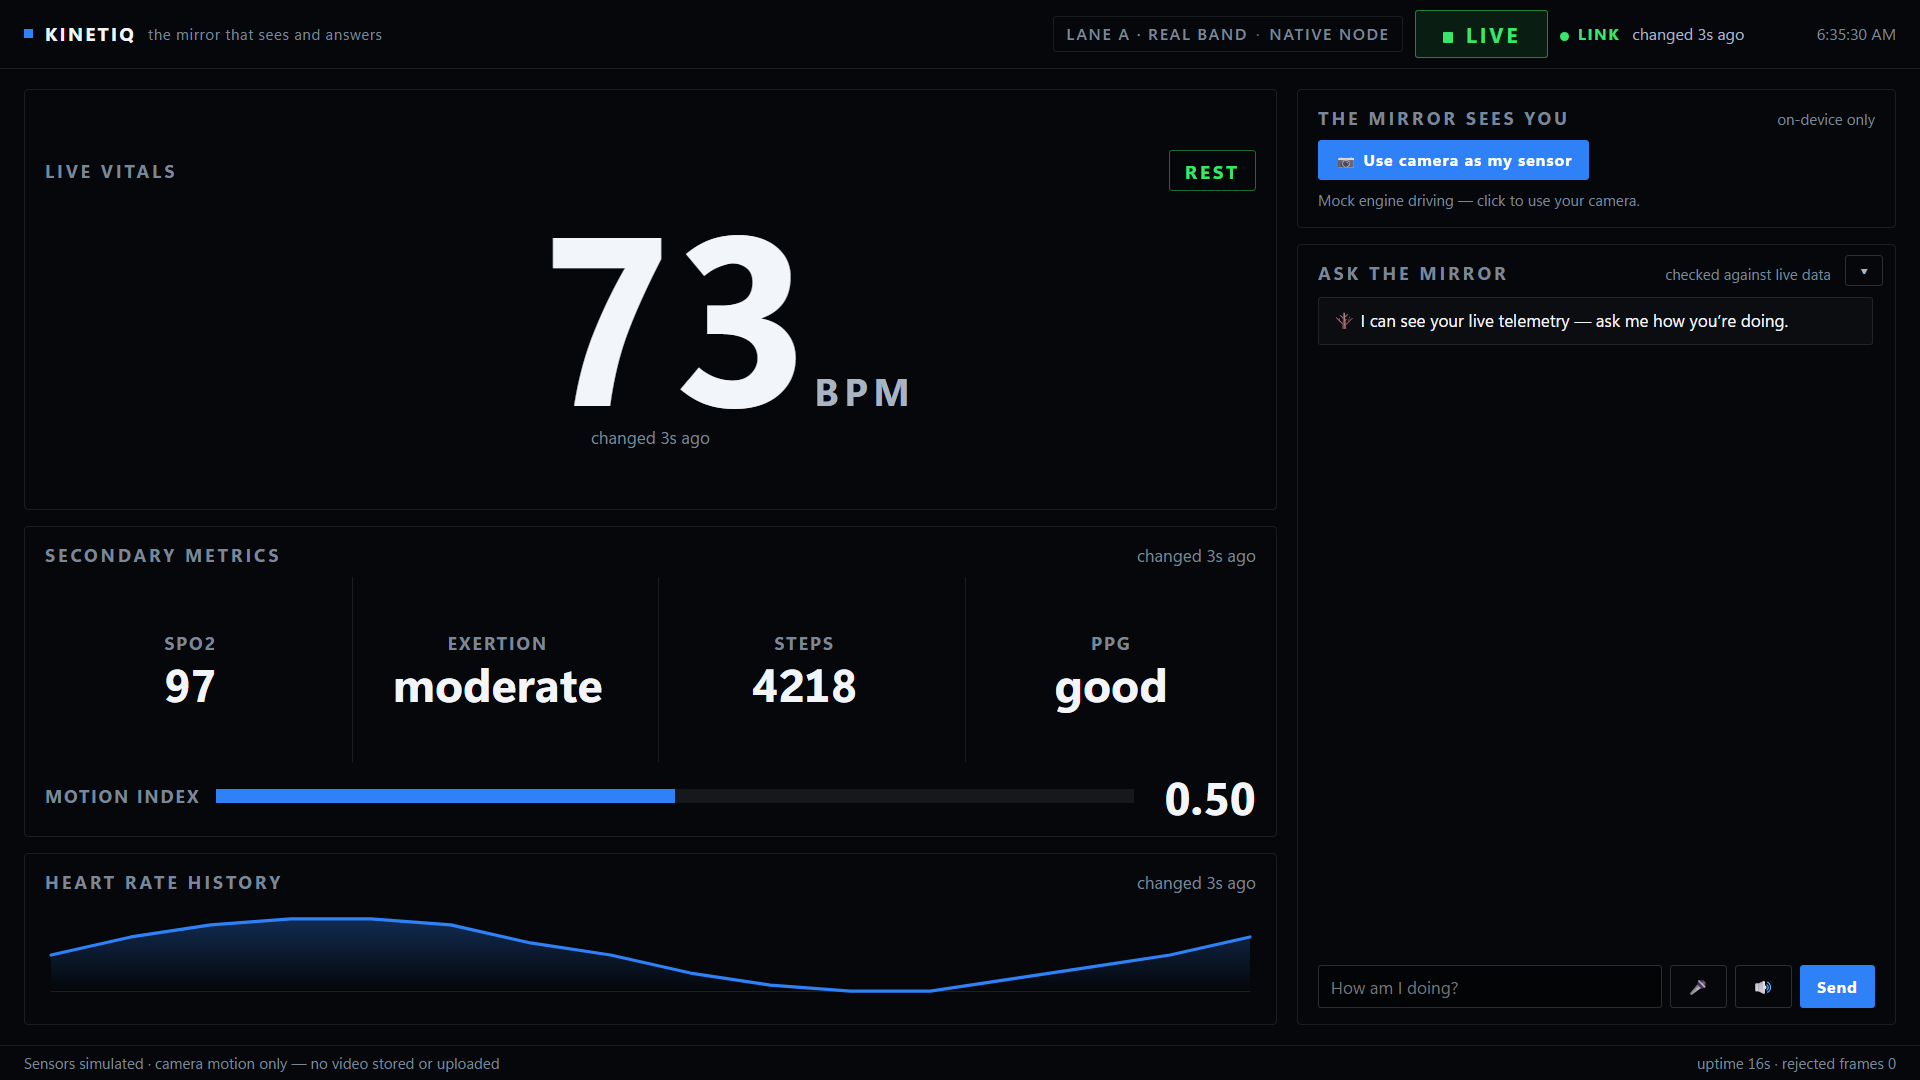
\includegraphics[width=\textwidth]{ui_live.png}
\caption[Dashboard mirror with synthetic stream (not live)]{Implemented dashboard mirror rendered in the browser during a controlled local input session; the displayed stream is synthetic, not live wearable telemetry.}
\label{fig:dashboard-live}
\end{figure}

The assistant accepts the current validated context, attempts a local Ollama \code{gemma2:2b} response where available, and otherwise uses a deterministic template. Responses are bounded to 70 words.

The verifier checks specified agreement with activity, exertion, an exact HR/heart value or step count, and poor-quality wording when applicable. The process shows \texttt{PASS} or \texttt{FAIL}; the examined implementation still sends text to speech after a failed check, so the verdict is informative rather than a fail-closed safety gate.

\section{Hardware Design Scope}
The selected embedded components are an ESP32 DevKit V1, MPU6050, HC-SR04, infrared sensor, DHT22, and supporting wiring/prototyping materials. The materials include pin mapping and a Wokwi sketch. Figure~\ref{fig:hardware-concept} reproduces the project material's earlier hardware-path diagram as a conceptual design reference. It is not used as evidence of final physical sensor acquisition.

\begin{figure}[H]
\centering
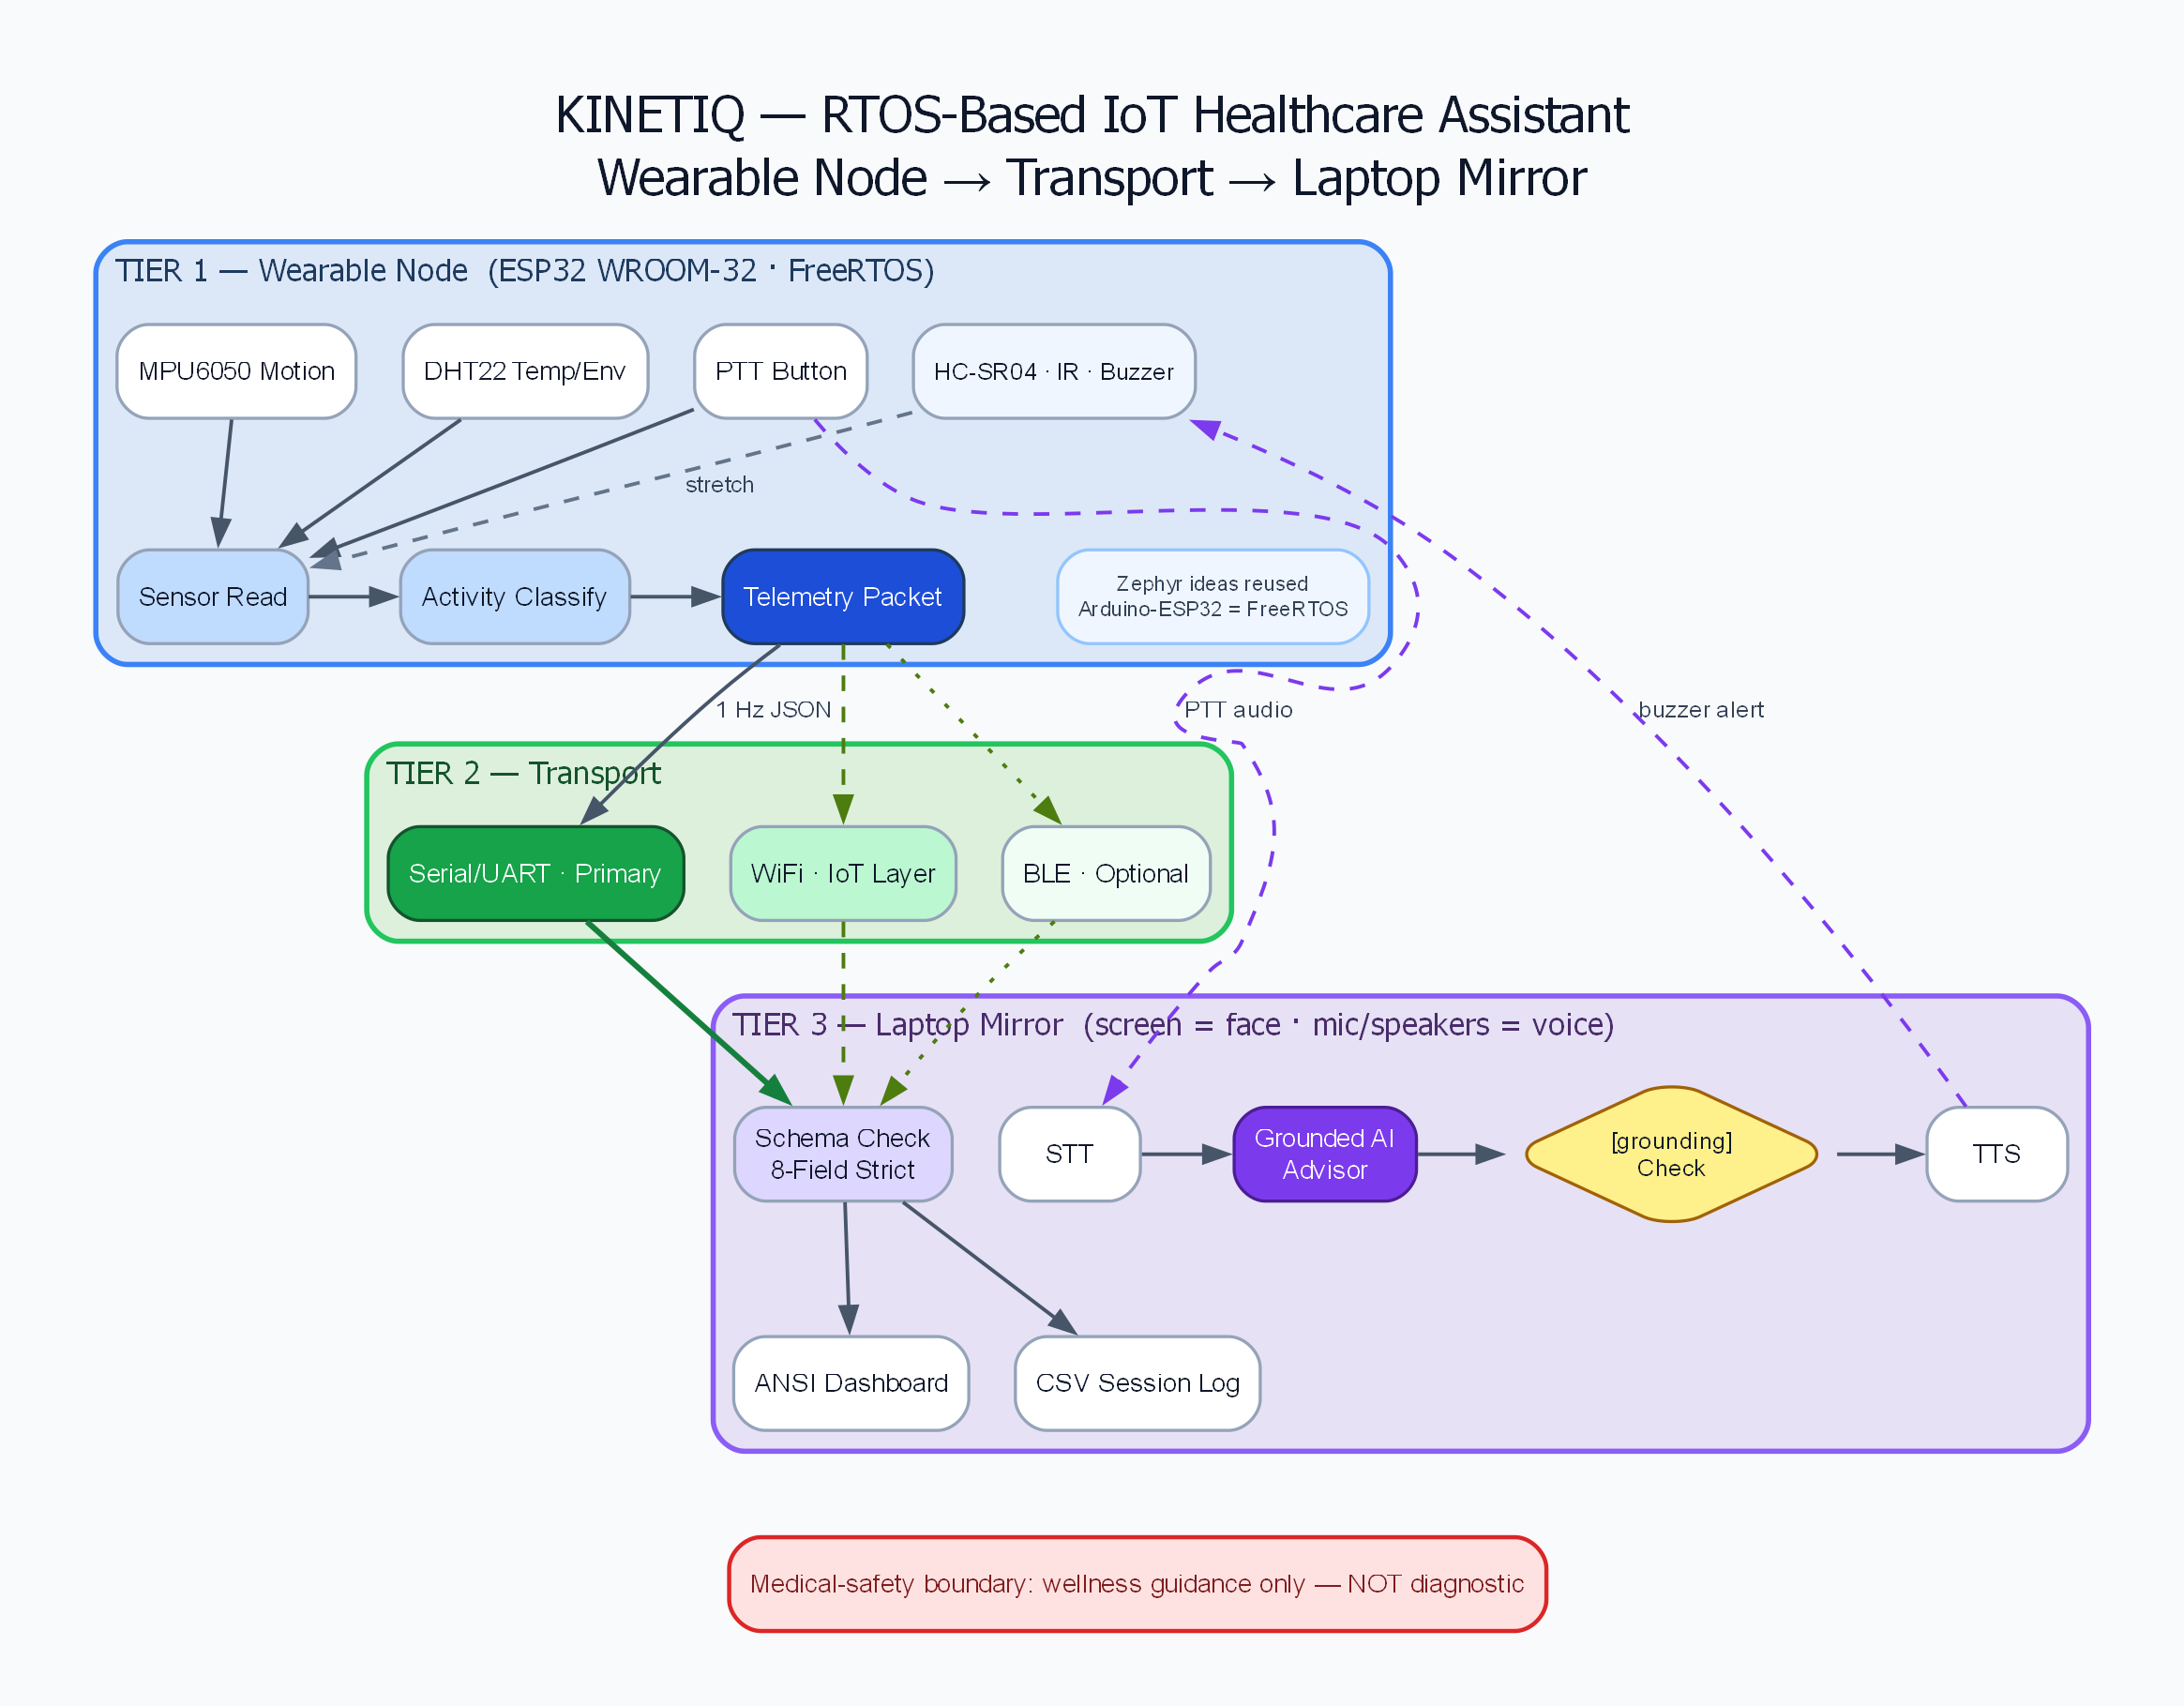
\includegraphics[width=0.82\textwidth]{existing_architecture.png}
\caption{Earlier hardware-path conceptual architecture from the KINETIQ project materials. The physical ESP32 sensing path remained planned/simulated at the documented final demonstration.}
\label{fig:hardware-concept}
\end{figure}

The ESP32 and sensor selection remains technically appropriate for a future sensing node, but physical wiring, calibration, power behaviour, environmental response, and end-to-end sensor ingestion require separate validation. Wokwi execution can exercise the modelled sketch, not replace those measurements.
